%% ---------------------------------------------------------------- Figures 2-7
\begin{figure}[!htbp]
\centering

\includegraphics[width=\linewidth]{figures/funnel.pdf}
\caption{\textbf{Architectures are removed before they are evaluated.} Raw design space,
survivors after structural and after bound-based elimination, and the number of
architectures actually handed to the evaluator, for four design-space scales and three
workload classes (logarithmic scale).}
\label{fig:ce:funnel}
\end{figure}

\begin{figure}[!htbp]
\centering
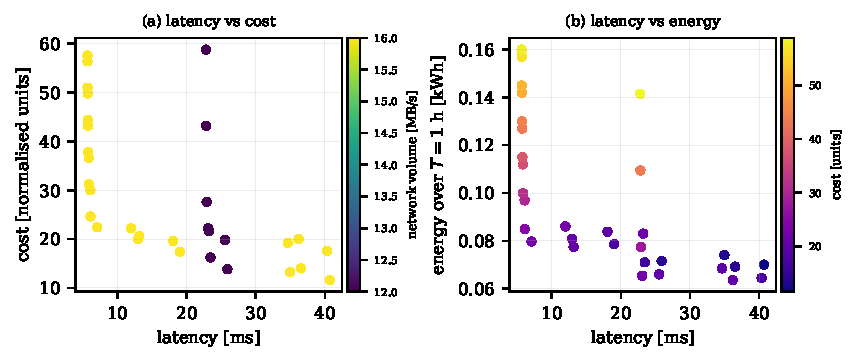
\includegraphics[width=\linewidth]{figures/pareto.pdf}
\caption{\textbf{The recovered set of optimal trade-offs.} Exact Pareto front on the
$51\,840$-candidate space for the telemetry workload. \textbf{a}, latency versus cost,
colour encodes network volume. \textbf{b}, latency versus energy over a one-hour horizon,
colour encodes cost.}
\label{fig:ce:pareto}
\end{figure}

\begin{figure}[!htbp]
\centering

\includegraphics[width=0.82\linewidth]{figures/crossover.pdf}
\caption{\textbf{The saving converts into time when evaluation is expensive.} Speed-up
over exhaustive enumeration projected from measured evaluation counts and measured
overheads as a function of the cost of one design-point evaluation. The dotted line marks
the measured cost of the discrete-event evaluator.}
\label{fig:ce:crossover}
\end{figure}

\begin{figure}[!htbp]
\centering

\includegraphics[width=\linewidth]{figures/hv_budget.pdf}
\caption{\textbf{Budget-matched stochastic exploration.} Hypervolume ratio against the
exhaustive front on the $51\,840$-candidate space over 20 seeds. Grey, random search;
blue, NSGA-II. The red line marks the exact front recovered by the proposed method.}
\label{fig:ce:hv}
\end{figure}

\begin{table}[!htbp]
\centering
\caption{\textbf{Budget-matched comparison.} Medians over 20 seeds at a budget of 1000
full evaluations; the full budget sweep is in Supplementary Tables~S1--S3.}
\label{tab:ce:base}
{\setlength{\tabcolsep}{3pt}\scriptsize
\begin{tabular}{lllrrrrr}
\toprule
scale & workload & method & evals & recall & HV ratio & IGD$^{+}$ & time [s] \\
\midrule

\multirow{4}{*}{S2} & \multirow{4}{*}{telemetry} & exhaustive & 3\,888 & 1.000 & 1.000 & 0.0000 & 0.044 \\
 & & random ($B$=1000) & 1000 & 0.259 & 0.927 & 0.0388 & 0.014 \\
 & & NSGA-II ($B$=1000) & 1000 & 0.926 & 0.999 & 0.0002 & 0.147 \\
 & & \textbf{HCA-DSE} & \textbf{44} & \textbf{1.000} & \textbf{1.000} & \textbf{0.0000} & 0.036 \\
\midrule
\multirow{4}{*}{S2} & \multirow{4}{*}{control} & exhaustive & 3\,888 & 1.000 & 1.000 & 0.0000 & 0.042 \\
 & & random ($B$=1000) & 1000 & 0.240 & 0.922 & 0.0377 & 0.014 \\
 & & NSGA-II ($B$=1000) & 1000 & 0.800 & 0.999 & 0.0030 & 0.160 \\
 & & \textbf{HCA-DSE} & \textbf{37} & \textbf{1.000} & \textbf{1.000} & \textbf{0.0000} & 0.035 \\
\midrule
\multirow{4}{*}{S2} & \multirow{4}{*}{sensing} & exhaustive & 3\,888 & 1.000 & 1.000 & 0.0000 & 0.029 \\
 & & random ($B$=1000) & 1000 & 0.250 & 0.897 & 0.0626 & 0.010 \\
 & & NSGA-II ($B$=1000) & 1000 & 0.875 & 1.000 & 0.0017 & 0.182 \\
 & & \textbf{HCA-DSE} & \textbf{26} & \textbf{1.000} & \textbf{1.000} & \textbf{0.0000} & 0.016 \\
\midrule
\multirow{4}{*}{S3} & \multirow{4}{*}{telemetry} & exhaustive & 34\,560 & 1.000 & 1.000 & 0.0000 & 0.308 \\
 & & random ($B$=1000) & 1000 & 0.032 & 0.732 & 0.1147 & 0.011 \\
 & & NSGA-II ($B$=1000) & 1000 & 0.500 & 0.946 & 0.0454 & 0.145 \\
 & & \textbf{HCA-DSE} & \textbf{50} & \textbf{1.000} & \textbf{1.000} & \textbf{0.0000} & 0.138 \\
\midrule
\multirow{4}{*}{S3} & \multirow{4}{*}{control} & exhaustive & 34\,560 & 1.000 & 1.000 & 0.0000 & 0.265 \\
 & & random ($B$=1000) & 1000 & 0.000 & 0.725 & 0.1189 & 0.010 \\
 & & NSGA-II ($B$=1000) & 1000 & 0.648 & 0.984 & 0.0236 & 0.147 \\
 & & \textbf{HCA-DSE} & \textbf{41} & \textbf{1.000} & \textbf{1.000} & \textbf{0.0000} & 0.125 \\
\midrule
\multirow{4}{*}{S3} & \multirow{4}{*}{sensing} & exhaustive & 34\,560 & 1.000 & 1.000 & 0.0000 & 0.266 \\
 & & random ($B$=1000) & 1000 & 0.000 & 0.658 & 0.1569 & 0.010 \\
 & & NSGA-II ($B$=1000) & 1000 & 0.741 & 0.951 & 0.1677 & 0.175 \\
 & & \textbf{HCA-DSE} & \textbf{43} & \textbf{1.000} & \textbf{1.000} & \textbf{0.0000} & 0.085 \\
\bottomrule
\end{tabular}
}
\end{table}

\begin{figure}[!htbp]
\centering

\includegraphics[width=0.7\linewidth]{figures/scalability.pdf}
\caption{\textbf{The design space is never materialised.} Expanded partial designs and
full evaluations against the raw design-space size, over five orders of magnitude.}
\label{fig:ce:scal}
\end{figure}

\begin{table}[!htbp]
\centering
\caption{\textbf{Independent deployment validation.} Analytical predictions against
measured run means over 36 architectures and 108 runs with the model frozen beforehand.
Pair agreement is the share of architecture pairs whose measured order matches the
predicted order among pairs separated by more than $25\%$. ALL pools workloads.}
\label{tab:ce:testbed}
\scriptsize
\small
\begin{tabular}{lrrrrr}
\toprule
workload & $n$ & MAPE [\%] & Spearman $\rho$ & agreement $>25\%$ & pairs \\
\midrule
telemetry & 12 & 17.8 & 0.776 & 0.895 & 38 \\
control & 12 & 12.0 & 0.865 & 0.886 & 44 \\
sensing & 12 & 46.3 & 0.921 & 0.913 & 23 \\
ALL & 36 & 25.4 & 0.967 & 0.978 & 498 \\
\bottomrule
\end{tabular}

\end{table}

\begin{figure}[!htbp]
\centering

\includegraphics[width=0.62\linewidth]{figures/testbed.pdf}
\caption{\textbf{Predicted against measured latency.} Analytical latency versus the
median of three measured mean latencies on the independent containerised deployment. Open
markers denote architectures whose repeated means differ by a factor of $1.5$ or more.}
\label{fig:ce:testbed}
\end{figure}
